\documentclass[conference,a4paper]{IEEEtran}



% *** CITATION PACKAGES ***
%
%\usepackage{cite}
% cite.sty was written by Donald Arseneau
% V1.6 and later of IEEEtran pre-defines the format of the cite.sty package
% \cite{} output to follow that of IEEE. Loading the cite package will
% result in citation numbers being automatically sorted and properly
% "compressed/ranged". e.g., [1], [9], [2], [7], [5], [6] without using
% cite.sty will become [1], [2], [5]--[7], [9] using cite.sty. cite.sty's
% \cite will automatically add leading space, if needed. Use cite.sty's
% noadjust option (cite.sty V3.8 and later) if you want to turn this off.
% cite.sty is already installed on most LaTeX systems. Be sure and use
% version 4.0 (2003-05-27) and later if using hyperref.sty. cite.sty does
% not currently provide for hyperlinked citations.
% The latest version can be obtained at:
% http://www.ctan.org/tex-archive/macros/latex/contrib/cite/
% The documentation is contained in the cite.sty file itself.






% *** GRAPHICS RELATED PACKAGES ***
%
\ifCLASSINFOpdf
  \usepackage[pdftex]{graphicx}
  \usepackage{placeins}
  % declare the path(s) where your graphic files are
  % \graphicspath{{../pdf/}{../jpeg/}}
  % and their extensions so you won't have to specify these with
  % every instance of \includegraphics
  % \DeclareGraphicsExtensions{.pdf,.jpeg,.png}
\else
  % or other class option (dvipsone, dvipdf, if not using dvips). graphicx
  % will default to the driver specified in the system graphics.cfg if no
  % driver is specified.
  % \usepackage[dvips]{graphicx}
  % declare the path(s) where your graphic files are
  % \graphicspath{{../eps/}}
  % and their extensions so you won't have to specify these with
  % every instance of \includegraphics
  % \DeclareGraphicsExtensions{.eps}
\fi
% graphicx was written by David Carlisle and Sebastian Rahtz. It is
% required if you want graphics, photos, etc. graphicx.sty is already
% installed on most LaTeX systems. The latest version and documentation can
% be obtained at: 
% http://www.ctan.org/tex-archive/macros/latex/required/graphics/
% Another good source of documentation is "Using Imported Graphics in
% LaTeX2e" by Keith Reckdahl which can be found as epslatex.ps or
% epslatex.pdf at: http://www.ctan.org/tex-archive/info/
%
% latex, and pdflatex in dvi mode, support graphics in encapsulated
% postscript (.eps) format. pdflatex in pdf mode supports graphics
% in .pdf, .jpeg, .png and .mps (metapost) formats. Users should ensure
% that all non-photo figures use a vector format (.eps, .pdf, .mps) and
% not a bitmapped formats (.jpeg, .png). IEEE frowns on bitmapped formats
% which can result in "jaggedy"/blurry rendering of lines and letters as
% well as large increases in file sizes.
%
% You can find documentation about the pdfTeX application at:
% http://www.tug.org/applications/pdftex





% *** MATH PACKAGES ***
%
%\usepackage[cmex10]{amsmath}
% A popular package from the American Mathematical Society that provides
% many useful and powerful commands for dealing with mathematics. If using
% it, be sure to load this package with the cmex10 option to ensure that
% only type 1 fonts will utilized at all point sizes. Without this option,
% it is possible that some math symbols, particularly those within
% footnotes, will be rendered in bitmap form which will result in a
% document that can not be IEEE Xplore compliant!
%
% Also, note that the amsmath package sets \interdisplaylinepenalty to 10000
% thus preventing page breaks from occurring within multiline equations. Use:
%\interdisplaylinepenalty=2500
% after loading amsmath to restore such page breaks as IEEEtran.cls normally
% does. amsmath.sty is already installed on most LaTeX systems. The latest
% version and documentation can be obtained at:
% http://www.ctan.org/tex-archive/macros/latex/required/amslatex/math/





% *** SPECIALIZED LIST PACKAGES ***
%
%\usepackage{algorithmic}
% algorithmic.sty was written by Peter Williams and Rogerio Brito.
% This package provides an algorithmic environment fo describing algorithms.
% You can use the algorithmic environment in-text or within a figure
% environment to provide for a floating algorithm. Do NOT use the algorithm
% floating environment provided by algorithm.sty (by the same authors) or
% algorithm2e.sty (by Christophe Fiorio) as IEEE does not use dedicated
% algorithm float types and packages that provide these will not provide
% correct IEEE style captions. The latest version and documentation of
% algorithmic.sty can be obtained at:
% http://www.ctan.org/tex-archive/macros/latex/contrib/algorithms/
% There is also a support site at:
% http://algorithms.berlios.de/index.html
% Also of interest may be the (relatively newer and more customizable)
% algorithmicx.sty package by Szasz Janos:
% http://www.ctan.org/tex-archive/macros/latex/contrib/algorithmicx/




% *** ALIGNMENT PACKAGES ***
%
%\usepackage{array}
% Frank Mittelbach's and David Carlisle's array.sty patches and improves
% the standard LaTeX2e array and tabular environments to provide better
% appearance and additional user controls. As the default LaTeX2e table
% generation code is lacking to the point of almost being broken with
% respect to the quality of the end results, all users are strongly
% advised to use an enhanced (at the very least that provided by array.sty)
% set of table tools. array.sty is already installed on most systems. The
% latest version and documentation can be obtained at:
% http://www.ctan.org/tex-archive/macros/latex/required/tools/


%\usepackage{mdwmath}
%\usepackage{mdwtab}
% Also highly recommended is Mark Wooding's extremely powerful MDW tools,
% especially mdwmath.sty and mdwtab.sty which are used to format equations
% and tables, respectively. The MDWtools set is already installed on most
% LaTeX systems. The lastest version and documentation is available at:
% http://www.ctan.org/tex-archive/macros/latex/contrib/mdwtools/


% IEEEtran contains the IEEEeqnarray family of commands that can be used to
% generate multiline equations as well as matrices, tables, etc., of high
% quality.


%\usepackage{eqparbox}
% Also of notable interest is Scott Pakin's eqparbox package for creating
% (automatically sized) equal width boxes - aka "natural width parboxes".
% Available at:
% http://www.ctan.org/tex-archive/macros/latex/contrib/eqparbox/





% *** SUBFIGURE PACKAGES ***
%\usepackage[tight,footnotesize]{subfigure}
% subfigure.sty was written by Steven Douglas Cochran. This package makes it
% easy to put subfigures in your figures. e.g., "Figure 1a and 1b". For IEEE
% work, it is a good idea to load it with the tight package option to reduce
% the amount of white space around the subfigures. subfigure.sty is already
% installed on most LaTeX systems. The latest version and documentation can
% be obtained at:
% http://www.ctan.org/tex-archive/obsolete/macros/latex/contrib/subfigure/
% subfigure.sty has been superceeded by subfig.sty.



%\usepackage[caption=false]{caption}
%\usepackage[font=footnotesize]{subfig}
% subfig.sty, also written by Steven Douglas Cochran, is the modern
% replacement for subfigure.sty. However, subfig.sty requires and
% automatically loads Axel Sommerfeldt's caption.sty which will override
% IEEEtran.cls handling of captions and this will result in nonIEEE style
% figure/table captions. To prevent this problem, be sure and preload
% caption.sty with its "caption=false" package option. This is will preserve
% IEEEtran.cls handing of captions. Version 1.3 (2005/06/28) and later 
% (recommended due to many improvements over 1.2) of subfig.sty supports
% the caption=false option directly:
%\usepackage[caption=false,font=footnotesize]{subfig}
%
% The latest version and documentation can be obtained at:
% http://www.ctan.org/tex-archive/macros/latex/contrib/subfig/
% The latest version and documentation of caption.sty can be obtained at:
% http://www.ctan.org/tex-archive/macros/latex/contrib/caption/




% *** FLOAT PACKAGES ***
%
%\usepackage{fixltx2e}
% fixltx2e, the successor to the earlier fix2col.sty, was written by
% Frank Mittelbach and David Carlisle. This package corrects a few problems
% in the LaTeX2e kernel, the most notable of which is that in current
% LaTeX2e releases, the ordering of single and double column floats is not
% guaranteed to be preserved. Thus, an unpatched LaTeX2e can allow a
% single column figure to be placed prior to an earlier double column
% figure. The latest version and documentation can be found at:
% http://www.ctan.org/tex-archive/macros/latex/base/



\usepackage{stfloats}
% stfloats.sty was written by Sigitas Tolusis. This package gives LaTeX2e
% the ability to do double column floats at the bottom of the page as well
% as the top. (e.g., "\begin{figure*}[!b]" is not normally possible in
% LaTeX2e). It also provides a command:
%\fnbelowfloat
% to enable the placement of footnotes below bottom floats (the standard
% LaTeX2e kernel puts them above bottom floats). This is an invasive package
% which rewrites many portions of the LaTeX2e float routines. It may not work
% with other packages that modify the LaTeX2e float routines. The latest
% version and documentation can be obtained at:
% http://www.ctan.org/tex-archive/macros/latex/contrib/sttools/
% Documentation is contained in the stfloats.sty comments as well as in the
% presfull.pdf file. Do not use the stfloats baselinefloat ability as IEEE
% does not allow \baselineskip to stretch. Authors submitting work to the
% IEEE should note that IEEE rarely uses double column equations and
% that authors should try to avoid such use. Do not be tempted to use the
% cuted.sty or midfloat.sty packages (also by Sigitas Tolusis) as IEEE does
% not format its papers in such ways.





% *** PDF, URL AND HYPERLINK PACKAGES ***
%
\usepackage{url}
% url.sty was written by Donald Arseneau. It provides better support for
% handling and breaking URLs. url.sty is already installed on most LaTeX
% systems. The latest version can be obtained at:
% http://www.ctan.org/tex-archive/macros/latex/contrib/misc/
% Read the url.sty source comments for usage information. Basically,
% \url{my_url_here}.

\newcommand{\shellcmd}[1]{\\\texttt{\footnotesize\# #1}\\}
% *** Do not adjust lengths that control margins, column widths, etc. ***
% *** Do not use packages that alter fonts (such as pslatex).         ***
% There should be no need to do such things with IEEEtran.cls V1.6 and later.
% (Unless specifically asked to do so by the journal or conference you plan
% to submit to, of course. )

\begin{document}
%
% paper title
% can use linebreaks \\ within to get better formatting as desired
\title{Application of the whole-body-control approach for a mobile robot with a manipulator}


% author names and affiliations
% use a multiple column layout for up to three different
% affiliations
\author{\IEEEauthorblockN{Bartosz Multan, Dawid Mościcki,\\Tomasz Walburg, Mateusz Witka-Jeżewski}
\IEEEauthorblockA{Faculty of Electronics, Telecomunications and Informatics\\
Gdańsk University of Technology}}

% conference papers do not typically use \thanks and this command
% is locked out in conference mode. If really needed, such as for
% the acknowledgment of grants, issue a \IEEEoverridecommandlockouts
% after \documentclass

% for over three affiliations, or if they all won't fit within the width
% of the page, use this alternative format:
% 
%\author{\IEEEauthorblockN{Michael Shell\IEEEauthorrefmark{1},
%Homer Simpson\IEEEauthorrefmark{2},
%James Kirk\IEEEauthorrefmark{3}, 
%Montgomery Scott\IEEEauthorrefmark{3} and
%Eldon Tyrell\IEEEauthorrefmark{4}}
%\IEEEauthorblockA{\IEEEauthorrefmark{1}School of Electrical and Computer Engineering\\
%Georgia Institute of Technology,
%Atlanta, Georgia 30332--0250\\ Email: see http://www.michaelshell.org/contact.html}
%\IEEEauthorblockA{\IEEEauthorrefmark{2}Twentieth Century Fox, Springfield, USA\\
%Email: homer@thesimpsons.com}
%\IEEEauthorblockA{\IEEEauthorrefmark{3}Starfleet Academy, San Francisco, California 96678-2391\\
%Telephone: (800) 555--1212, Fax: (888) 555--1212}
%\IEEEauthorblockA{\IEEEauthorrefmark{4}Tyrell Inc., 123 Replicant Street, Los Angeles, California 90210--4321}}




% use for special paper notices
%\IEEEspecialpapernotice{(Invited Paper)}




% make the title area
\maketitle


\begin{abstract}
This paper deals with the issue of a whole-body-control approach for a mobile robot with a manipulator.
The goal of the project was to design a whole-body-control algorithm, which would allow the robot to perform pick and place tasks autonomously.
The work contains a description of used algorithms such as Dex-Net, YOLO or SLAM. The process of integration of all system components was discussed.
The outcomes of the preformed simulation were presented.
The achieved results as well as encountered problems were also described.
\end{abstract}
% IEEEtran.cls defaults to using nonbold math in the Abstract.
% This preserves the distinction between vectors and scalars. However,
% if the conference you are submitting to favors bold math in the abstract,
% then you can use LaTeX's standard command \boldmath at the very start
% of the abstract to achieve this. Many IEEE journals/conferences frown on
% math in the abstract anyway.

\begin{IEEEkeywords}
mobile robot, robotic arm, object detection, ROS, whole-body-control, YOLO
\end{IEEEkeywords}



% For peer review papers, you can put extra information on the cover
% page as needed:
% \ifCLASSOPTIONpeerreview
% \begin{center} \bfseries EDICS Category: 3-BBND \end{center}
% \fi
%
% For peerreview papers, this IEEEtran command inserts a page break and
% creates the second title. It will be ignored for other modes.
\IEEEpeerreviewmaketitle


\section{Introduction}

The whole-body-control approach is a method for controlling the motion of a robot by considering the interactions between the robot's various components, such as its base, manipulator, and sensors. The goal of whole-body control is to coordinate the motion of the robot's different parts to achieve a specific task or set of tasks, while also taking into account the robot's dynamic constraints and environmental factors.
The whole-body control approach is distinct from traditional control methods, which typically focus on controlling the motion of individual components, such as the joints of a manipulator, in isolation. By contrast, whole-body control considers the robot as a holistic system and seeks to coordinate the motion of its different parts to achieve a more efficient, stable, and safe motion.

This approach allows the robot to achieve a greater degree of flexibility and versatility in its movements. Also, it enables the possibility to perform more complicated pick and place tasks.

To implement a whole-body-control algorithm there was a need for the integration of various sub-systems. A vision system with the ability to detect and distinguish objects was necessary. For this purpose, the presented result uses the YOLO algorithm. To perform a grasping action in a pick and place task Dex-Net algorithm was used. What is more to define the robot's position LiDAR sensor and RGBD camera were integrated. 

In this paper the challenges that were encountered during the implementation of the approach and the solutions that were developed to overcome them were described. 
The results of experiments conducted to evaluate the performance of the whole-body-control approach were also presented and discussed.

\subsection{Simulation environment and robots used in experiment} 
To perform integration and tests, Gazebo and Robot Operating System were choosen. As a holonomic mobile platform Clearpath Dingo robot has been used. As a manipulator with 7 DoF,  to provide wide range of possible movements Panda Franka Emika has been choosen.

\subsection{Sensor selection}
Sensor selection involves considering various different aproaches for subtasks needed to achieve main goal.

Four main subtasks were:
\begin{itemize}
  \item Localisation and mapping
  \item Object Recognition
  \item Graps point definition
  \item Grabbing
\end{itemize}

First three tasks are essential in term of sensor selection, because grabbing alone could be performed based on \textit{a priori} gained data. Also, sensors which are commonly used to aquire Object Recognition and Graps point definition are simmilar so they will be present in common subsection.

\subsubsection{Localisation and mapping}
Localisation and mapping is crucial when it comes to going through the environment and there are three approaches. First is using 2d lidar sensor, which gives information about obstacles on 2d plane. It is efficient and easy to implement and in  singular-level buildings and without 
ability to go under the obstacles - completely adequate. If we would like to allow robot to go over (i.e. drones) it could be better to use 3d laser scanners (which give a point cloud data which allows to map 3d environment) or RGBD cameras which allow to create 
pointcloud with limited field of view and perform computer vision at the same time.

To perform localisation and mapping, Sick LMS1xx 2D Lidar and Intel Realsense RGBD camera were used as a source of both 2D laser scan information and 3d pointcloud and rgb image. It provides possibility of using visual odometry to calculate difference in robot's pose i


\subsubsection{Object Recognition and Graps point definition}
To recognise objects, it is necessary to have their rgb image, which has to be captured by the camera. 
To define grabbing point it is important to have the rgb data and pointcloud to perform shape recognition. To meet both dependencies, it has been decided to use Realsense RGBD camera which has good implementation in Gazebo. Even though Realsense does not provide pointcloud data directly, it can be 
computated from rgb image and depth image.

To allow robot to see objects from manipulator perspective, one Realsense camera was placed close to the efector ending.

\section{Autonomous driving}
To aquire autonomous driving in indoor environment, system consisted of two main parts - localisation and mapping algorithm and motion planner algorithm.

The structure of the system has been presented in Figure 1.

\begin{figure}[ht]
  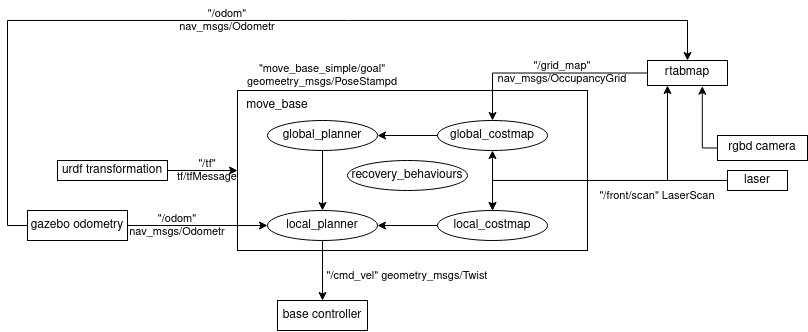
\includegraphics[width=0.5\textwidth]{img/navigation_scheme.png}
  \caption[navigation structure]{Autonomous driving system}
\end{figure}

\subsection{Simultaneous Localisation and Mapping}
To achieve mapping and localisation for mobile platform, RTABMAP (Real Time appearance Based Mapping) \cite{RTABMAP} was choosen as a effective algorithm to implement 3D slam with loop closure detection. It uses lidar \textit{LaserScan} messages from Sick lidar and rgb image and depth image from Realsense camera to create 2d grid map used for navigation and 3d pointcloud presenting the surrounding environment. 
As an odometry source, it has been decided to use odometry information given by the Gazebo simulator because of the most efficient way of getting odometry in terms of computation power needed performing simulation.

\subsection{Motion planner}
To move the platform in simulated environment, it has been decided to use \textit{move\_base} package with global planner \textit{NavfnROS} and local planner \textit{TrajectoryPlanner ROS}. \textit{NavfnROS} is an implementation of fast, interpolated navigation function used to create paths to the target position.  \textit{TrajectoryPlanner ROS} is a local planner with creates set of different trajectories with kinematic constraints
and scores them in terms of how close they are to the created global path. Local plan with the highest score is the send to the base controller as a \textit{geometry message}.
Octomap was considered as an extension of the system to calculate the possibility of going under the obstacles such as tables but it has not been implemented. 

\begin{figure}[ht]
  \centering
  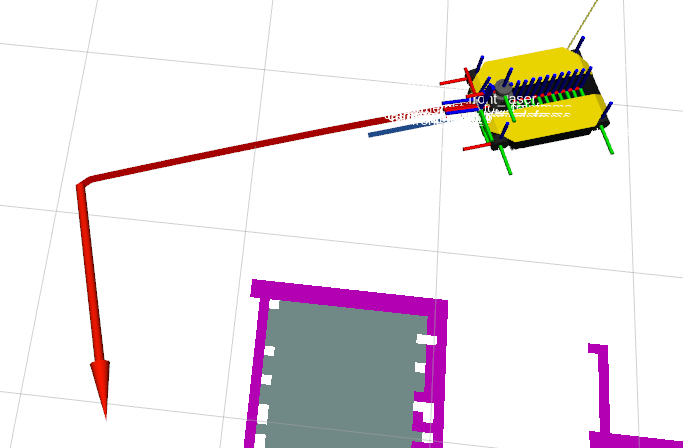
\includegraphics[width=0.4\textwidth]{img/global_local_planner.png}
  \caption[global and local path]{Goal position (red arrow), global path (red line) and local path (blue line)}
\end{figure}
\FloatBarrier


\section{Manipulator control}
To control Panda Franka Emika, which is 7 DoF robotic arm, it has been decided to use MoveIt. MoveIt is a Motion Planning Framework integrated with Robot Operating System. It is primarily used for mobile manipulation and grasping tasks, and can be integrated with various robot platforms and sensor systems. MoveIt provides a high-level interface for controlling a robot's motion, and includes features such as motion planning, collision detection, and visualization tools \cite{MOVEIT}.
MoveIt uses IKFast the Roboti Kinematics Compiler which is a powerful inverse kinematics solver. 

\section{Object recognition}
In this section YOLO algorithm was described, which was used for object recogniton task. This section also contains a decryption of a process of integrating and installing dark-net ROS package \cite{YOLO_ROS}.

\subsection{Algorithm description}
YOLO (You Only Look Once) is a real-time object detection algorithm. YOLO contains single convolutional neural network (CNN) that is able to detect objects in an image or video stream in real-time. 

The YOLO algorithm divides the input image into a grid of cells, and for each cell, it predicts a set of bounding boxes and their corresponding class probabilities. Each bounding box is represented by a set of four numbers, which denote the coordinates of the top-left corner and the bottom-right corner of the box. The class probabilities are represented by a set of numbers, one for each class in the dataset.

YOLO algorithm is known for its fast detection speed, and good accuracy-speed trade-off compared to other methods such as R-CNN (Region-based Convolutional Neural Networks) or DPM (Deformable Part Model) \cite{YOLO_paper}. However, the YOLO algorithm has some limitations, such as its tendency to miss small objects and its lack of rotation invariance. This nonetheless was not the issue in the application of the YOLO algorithm in the project. 

\subsection{Used dataset}
YOLO algorithm used in the project is trained on COCO dataset. Based on that dataset YOLO can detect 80 object classes.
\begin{itemize}
\item person
\item bicycle, car, motorbike, aeroplane, bus, train, truck, boat
\item traffic light, fire hydrant, stop sign, parking meter, bench
\item cat, dog, horse, sheep, cow, elephant, bear, zebra, giraffe
\item backpack, umbrella, handbag, tie, suitcase, frisbee, skis, snowboard, sports ball, kite, baseball bat, baseball glove, skateboard, surfboard, tennis racket
\item bottle, wine glass, cup, fork, knife, spoon, bowl
\item banana, apple, sandwich, orange, broccoli, carrot, hot dog, pizza, donut, cake
\item chair, sofa, pottedplant, bed, diningtable, toilet, tvmonitor, laptop, mouse, remote, keyboard, cell phone, microwave, oven, toaster, sink, refrigerator, book, clock, vase, scissors, teddy bear, hair drier, toothbrush
\end{itemize}

\subsection{Installation and integration}
To run YOLO object detection package OpenCV and boost libraries are needed. Also, before running YOLO algorithm pretrained weights should be downloaded. There are two possible options: weights for YOLO tiny and regular weights. Weights for YOLO tiny are used in smaller model, which is substantially faster, but less accurate. The weights can be downloaded by running a command:
\shellcmd{wget http://pjreddie.com/media/files/yolov3.weights}
After dowladnig weights the package can be run by a following command:
\shellcmd{roslaunch darknet\_ros darknet\_ros.launch}
In order to integrate the package with the project there was a need to modify ros.yml file and change camera\_reading topic to \url{/camera/color/image_raw}.

\subsection{Object detection results}
Integrated tiny version YOLO algorithm works correctly under certain conditions. The object must be specified in the dataset. What is more, the background and the lightning conditions should be appropriate. The tiny version of the algorithm uses less computing power, but it is less accurate in its predictions. The result of detecting an object is shown in a figure below. 

\begin{figure}[!ht]
  \centering
  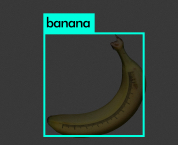
\includegraphics[width=0.2\textwidth]{img/Yolo_banana.jpeg}
  \caption{Detecting a banana using YOLO algorithm.}
\end{figure}

\section{Grasp detection}
This section describes the problems our team encountered when implementing the grasp detection algorithms into the project.

\subsection{Dex-Net and GQC Neural Networks}
Dex-Net and GQCNN packages are well suited for both Python, and ROS environment. While Dex-Net focuses on generating datasets of grasp robustness, the GQCNN is based on the Grasp Quality Convolutional Neural Networks which finds the best grasp from a group of candidates. Structure of this system has been shown below.

\begin{figure}[ht]
  \centering
  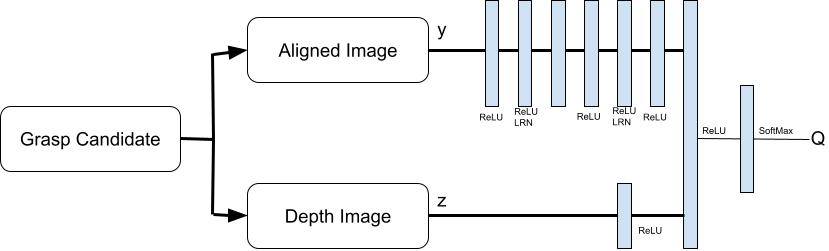
\includegraphics[width=0.47\textwidth]{img/gqcnn.png}
  \caption{Structure of Grasp Quality Concolutional Neural Network}
\end{figure}

Dex-Net is the library that has seen the most progress during the tests. It was run and tested using a high-level Python programming language. Unfortunately, though, issues occurred during its integration into the ROS environment.

\subsection{MoveIt Deep Grasps}
MoveIt Deep Grasps is a ROS package developed by Picknik.ai. It is a more advanced version of the MoveIt Grasps library. The package uses three tools:

\begin{itemize}
\item Grasp Pose Detection
\item Dex-Net
\item MoveIt Task Constructor
\end{itemize}

The MoveIt Task Constructor is used to ensure ROS communication with the decision-making system, which can be either Dex-Net or Grasp Pose Detection package. Both libraries must be installed on the computer before installing the ROS MoveIt Deep Grasps package.

During the installation process, many problems have occurred. With time, most of them have been resolved, however two issues could not have been fixed. It revolved around the compatibility of the OpenCV version, used by MoveIt Deep Grasps. Another error that was not resolved was the absence of certain files in the package itself.

\subsection{MoveIt Grasps}
MoveIt Grasps is yet another package designed for a Robot Operating System, maintained by the aforementioned Picknik.ai. Its main task is to generate grip points for simple objects, such as blocks and cylinders. This package is continuation of the MoveIt pick and place library. It is also the most popular package for grasp detection.

Attempts of installing the package have failed due to file compatibility issues. Extensive research has shown that due to MoveIt changes made in 2021, the package could no longer be supported. As a result, it became impossible to use it in our version of software.

\section{Whole body motion control algorithm}
For the purpose of this experiment, let assume that the approximate location of the desired object is known and it has been added to the map as a label. Then, next steps for the algorithm are as presented below.

\begin{figure}[ht]
  \centering
  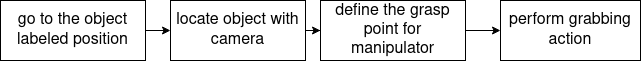
\includegraphics[width=0.5\textwidth]{img/algorithm_no_problem1.png}
  \caption{Sequence of achieving the task}
\end{figure}

Grabbing action should also be extended to measure the distance from the base\_link of the object and execute the base movement if it is necessary. To maintain all states and autonomy, the state node has been proposed with configuration showed below.

Autonomy actions would be maintained by \textit{state\_controller} node which could have structure presented below.
\begin{figure}[ht]
  \centering
  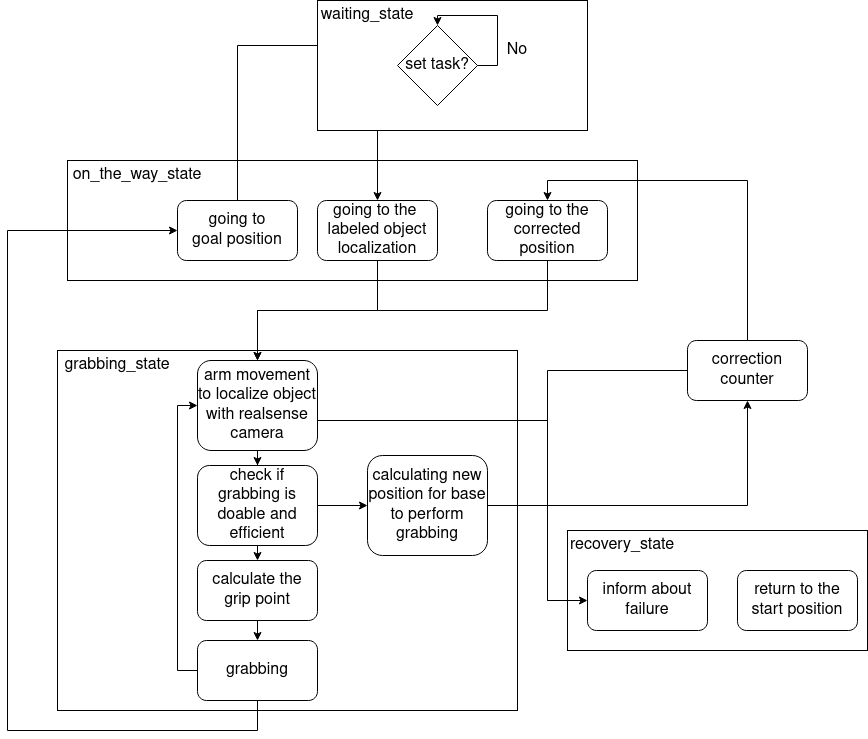
\includegraphics[width=0.5\textwidth]{img/states.png}
  \caption[states controller structure]{States controller concept}
\end{figure}
\FloatBarrier

\section{Difficulties}
During developing whole system, many diffculties occured. Implementation problems prevented completing the task of creating whole-body-motion control algorithm due to some significant unresolved errors.

\subsection{Integrating Dingo and Panda}
During integrating mobile robot Dingo with robotic arm Panda first step was to create common \textit{URDF} file to connect both robots together. However, for the simulation purposes, all movable parts have to be described by \textit{Hardware\_Interface}
and placed in common set. Because of the written drivers, with checking number of joints it was impossible to run the simulation. After changing the condition values, it turned out that Gazebo simulator is not able to control more sets of \textit{Hardware\_Joints}
than one because of the namespace conflict. Probably it could be repaired by rewritting part of the Panda driver, but it was too time consuming to perform succesfully.

\section{Conclusion}
The conclusion goes here.

% use section* for acknowledgement
\section*{Acknowledgment}


The authors would like to thank...



% trigger a \newpage just before the given reference
% number - used to balance the columns on the last page
% adjust value as needed - may need to be readjusted if
% the document is modified later
%\IEEEtriggeratref{8}
% The "triggered" command can be changed if desired:
%\IEEEtriggercmd{\enlargethispage{-5in}}

% references section

% can use a bibliography generated by BibTeX as a .bbl file
% BibTeX documentation can be easily obtained at:
% http://www.ctan.org/tex-archive/biblio/bibtex/contrib/doc/
% The IEEEtran BibTeX style support page is at:
% http://www.michaelshell.org/tex/ieeetran/bibtex/
%\bibliographystyle{IEEEtran}
% argument is your BibTeX string definitions and bibliography database(s)
%\bibliography{IEEEabrv,../bib/paper}
%
% <OR> manually copy in the resultant .bbl file
% set second argument of \begin to the number of references
% (used to reserve space for the reference number labels box)
\begin{thebibliography}{1}

\bibitem{RTABMAP}
M. Labbé and F. Michaud, “RTAB-Map as an Open-Source Lidar and Visual SLAM Library for Large-Scale and Long-Term Online Operation,” in Journal of Field Robotics, vol. 36, no. 2, pp. 416–446, 2019. 

\bibitem{MOVEIT}
David Coleman, Ioan A. Șucan, Sachin Chitta, Nikolaus Correll, Reducing the Barrier to Entry of Complex Robotic Software: a MoveIt! Case Study, Journal of Software Engineering for Robotics, 5(1):3–16, May 2014. doi: 10.6092/JOSER\_2014\_05\_01\_p3.

\bibitem{YOLO_ROS}
M. Bjelonic "YOLO ROS: Real-Time Object Detection for ROS", URL: \url{https://github.com/leggedrobotics/darknet_ros}, 2018.

\bibitem{YOLO_paper}
J. Redmon, S. Divvala, R. Girshick and A. Farhadi, "You Only Look Once: Unified, Real-Time Object Detection," 2016 IEEE Conference on Computer Vision and Pattern Recognition (CVPR), Las Vegas, NV, USA, 2016, pp. 779-788, doi: 10.1109/CVPR.2016.91.

\end{thebibliography}




% that's all folks
\end{document}


